\chapter{Systementwurf}\label{chp:systementwurf}


%#######################################################################################
%#######################################################################################
\section{Variantenmanagement und Parameter}
\paragraph{}

Die Lösung zum Speichern und Darstellen der Parameterwerte abhängig der aktiven Variante wird im diesem Kapitel erläutert.\\

\begin{figure}[h!]
  \begin{center}
    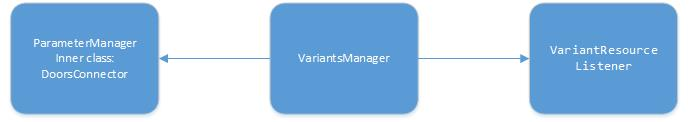
\includegraphics[scale=0.7]{5_1_klassenuebersicht.jpg}
  		  \caption{Einfache Übersicht der Klassen}
     \label{ttn.verbindung.klassen.loesung}
  \end{center}
\end{figure}


Um eine genauere Darstellung aller Klassen, bitte siehe Anhang \ref{A.PM.Diagramm}. Der Ablauf für das Speichern eines Parameters in einem Baumelement sieht folgendermaßen aus:
\begin{enumerate}
\item Benutzer verknüpft eine Anforderung an einem Baumelement
\item Der \textit{Listener} meldet das eine Änderung vorgenommen wird und gibt die Informationen weiter
\item Der \textit{VariantsManager} lädt und übergibt die nötige Informationen an das \textit{ParameterManager}
\item Der \textit{ParameterManager} lädt, sucht und erstellt ein \textit{ParameterTag}  und gibt das Befehl, dass ein \textit{ParameterTag} an ein Baumelement hinzugefügt werden muss.
\item Der \textit{ParameterManager} gibt das Befehl an das \textit{Listener} weiter
\item Das Befehl wird an die Befehlskette angehängt
\end{enumerate}

In den nächsten Unterkapiteln wird die Aufgaben der jeweiligen Klassen erläutert und der Ablauf ausführlicher erklärt.


%#######################################################################################
\subsection{VariantsManager}\label{sub.VariantsManager}
Die Hauptaufgabe des \textit{VariantsManager} ist die Varianten zu Zuordnen. Hier werden Baumelemente zu Varianten hinzugefügt und gelöscht. Dabei muss das Klassifikationsbaum neu gezeichnet werden. Diese Klasse kümmert sich auch, um die Umschaltung zwischen Varianten in der Variantenansicht (siehe Abbildung \ref{ttn.generic}) und die Richtige Darstellung der Baumelemente mit aktuelle Informationen.\\


Für die  Zwecke dieser Arbeit, wurde diese Klasse erweitert. Um die Aufgaben dieser Klasse zu erläutern, wird der Vorgang des Hinzufügen eines Parameters an einem Baumelement dargestellt. Der \textit{VariantsManager} setzt die Baumelement - ID und die Anforderungskennung in der Klasse \textit{ParameterManager}. Die Klasse dient als Schnittstelle zwischen der \textit{Listener} (siehe Kapitel \ref{sub:RSListner}) und die Klasse \textit{ParameterManager}  (siehe Kapitel \ref{sub:ParameterManager}).\\


Die Aufgabe des \textit{Listeners} lautet, dem \textit{VariantsManager} zu melden, wenn Änderung\footnote{Aktionen werden vom Benutzer ausgelöst anhand von Bedienelemente in der Benutzeroberfläche} geschehen werden oder geschehen sind. Im \textit{Listener} werden die benötigte Informationen gefiltert und an dieser Klasse weitergegeben, damit Änderung vorgenommen werden können. Im Fall der Parameterersetzung sind es die Identifikationsnummer eines Baumelementes und die Anforderungskennung der verlinkte Anforderung. Diese beide Kennungen diesen dazu, dass der \textit{VariantsManager} die jeweiligen Objekte (ein Baumelement und eine Anforderung) laden kann. Diese Objekte werden dann an der Klasse \textit{ParameterManager} übergeben.\\


Das angesprochene Baumelement muss aus das TESTONA-Diagramm geladen werden. Anhand der Identifikationsnummer werden die verschiedene Baumelemente einzeln abgefragt bis das richtige Baumelement gefunden wurde. Danach wird das Baumelement an das ParameterManager Objekt übergeben.\\


Im Fall von der Anforderungskennung, werden mehrere Informationen übergeben. Die Anforderungskennung wird in einer lokalen Variable vom ParameterManager Objekt gespeichert. Damit der Inhalt der Anforderung gelesen werden kann, müssen alle in TESTONA gespeicherte Anforderung an das ParameterManager-Objekt übergeben werden. Die gespeicherten \textit{Tags} in das TESTONA Objekt werden abfragt um folgende Objekte an das ParameterManager Objekt zu übergeben:


\begin{itemize}
\item \textbf{RequirementsConnetionTag}: beinhaltet die Information zur Datenbankverbindung, unter anderem die Verbindungsidentifikation (DOORS), das Modul(Tabelle) wo die Anforderung gespeichert ist und die Schnittstelle zur Datenbank. Anhand dieser Informationen wird die Verbindung zur Datenbank später aufgebaut.
\item \textbf{RequirementsListTag}: ist eine \textit{Map} mit alle in TESTONA gespeicherten Anforderungen. Das \textit{Key} ist die Anforderungsidentifikationsnummer und der Wert der Inhalt der Anforderung. Eine Anforderung aus dieser Liste wurde an das Baumelement verknüpft.
\item \textbf{VariantListTag}: eine Liste mit alle in TESTONA definierten Varianten.
\end{itemize}


Anhand dieser Informationen kann die Klasse \textit{ParameterManager} ein Parameter an ein Baumelement hinzufügen. Parameter können nicht nur hinzugefügt werden, sondern aus gelöscht werden. Ein Parameter wird aus einem Baumelement gelöscht, indem die verknüpfte Anforderung vom Baumelement entfernt wird. Der Ablauft für das Löschen eines Parameter ist im Grunde der gleiche als beim hinzufügen. Zunächst werden die Funktionen des \textit{Listeners} erörtert.




%#######################################################################################
\subsection{ResourceSetListener}\label{sub:RSListner}
Das auslösendes Element ist, dass der Benutzer eine Anforderung mit einen Baumelement verknüpft. Um dieses Geschehen abzufragen muss ein \textit{Listener} programmiert werden, dass das Interface \textit{ResourceSetListener}\footnote{http://download.eclipse.org/modeling/emf/transaction/javadoc/1.0.3/org/eclipse/emf/transaction/ResourceSetListener.html} implementiert. Da dass \textit{VariantsManager} ein solcher \textit{Listener} bereits besitzt, wurde dieser erweitert. Die Aufgabe des \textit{ResourceSetListener} ist, dem Benutzer zu benachrichtigen, wenn sich eine Ressource ändert. Das \textit{Listener}  \glqq hört\grqq~ auf die reinkommenden Nachrichten (\textit{ResourceSetChangeEvent}) und wertet den Inhalt dieses Events aus.\\

Das \textit{Listener} implementiert zwei Methoden die für das Abfragen der Events relevant sind. Eine davon heißt \textit{resourceSetChanged(Event e)}. Diese Methode wird aufgerufen, wenn sich eine Ressource ändert. Am Anfang wurde diese Methode  für das Abhören von Events (wenn eine Anforderung zu einem Baumelement verknüpft wird) favorisiert um danach die Parameterersetzung zu triggern. Nach der Implementierung konnte ich feststellen, dass die Methode keine Schreibrechte auf die Baumelemente besitzt. Da die Ressource zu diesem Zeitpunkt sich schon geändert hat.\\


Um die Schreibrechte zu besitzen, wurde dann die Methode \textit{transactionAboutToCommit(Event e)} betrachtet. Diese Methode wird aufgerufen bevor eine Änderung geschieht. Es wird benachrichtigt, dass eine Änderung geschehen wird und welche Objekte (ein Baumelement und die angehängte Anforderung) betrachtet werden. Zu diesem Zeitpunkt besitzt die Klasse noch Schreibrechte auf die Baumelemente und kann Änderung vornehmen. Außerdem hat die Methode als Rückgabewert ein \textit{Command}. So können Kommandos an das Commandstack angekettet werden. Das Befehl, ein Parameter an ein Baumelement hinzufügen, wird zum richtigen Zeitpunkt ausgeführt, dank der Anordnung des Commandstacks. Mehr zu Kommandos wird in Kapitel \ref{sub.Command} erwähnt.


Die empfangene Nachricht beinhaltet folgende Elemente: 

\begin{itemize}
\item \textbf{Event: }ResourceSetChangeEvent, die Ressourcen des Objektes haben sich geändert
\item \textbf{Notifier: } welches Objekt schickt die Nachricht
\item \textbf{Notification: }Beschreibung von der Änderung im \textit{Notifier}
\item \textbf{OldValue: } alter Wert, wenn nicht vorhanden \textit{null}
\item \textbf{NewValue: } neuer Wert, beim löschen von Werten \textit{null}
\end{itemize}


Hier wird als erstes der \textit{Notifier} abgefragt um auswerten zu können, ob die Nachricht relevant ist. Es gibt drei Fälle das unterscheiden werden müssen. Eine Anforderung wird:


\begin{enumerate}
\item zum ersten Mal an einem Baumelement verknüpft
\item an einem Baumelement verknüpft, wo schon ändere Anforderungen verknüpft sind
\item gelöscht
\end{enumerate}


Für alle drei Fälle muss der \textit{Listener} wissen, an welches Element wurde das Event ausgelöst und welche Anforderung wurde hinzugefügt oder gelöscht. Zu bemerken ist, dass zu diesem Zeitpunkt noch nicht festgestellt werden kann, ob in der Anforderung ein Parameter definiert ist.\\


\subsubsection{Eine Anforderung hinzufügen}
Ist der \textit{Notifier} eine Instanz von \textit{TestonaClass}, so wurde eine Anforderung zum ersten mal an ein Baumelement verknüpft oder gelöscht. Um Unterscheiden zu können werden die Werte von \textit{NewValue} und \textit{OldValue} ausgewertet. Wenn \textit{NewValue} eine Instanz von \textit{RequirementTag} ist, dann wurde eine Anforderung hinzugefügt. Aus dem \textit{Notifier} wird die ID (repräsentiert das Baumelement) und aus der Variable \textit{NewValue} die Anforderungskennung (diese wurde in DOORS vergeben) abgefragt. Beide Werte werden an dem \textit{Variantsmanager} weitergegeben um danach der Befehl als Rückgabewert für das hinzufügen eines \textit{ParameterTags} zu bekommen.\\


Der Befehl wird nicht sofort als Rückgabewert der Methode \textit{transactionAboutToCommit} weitergegeben. Der Grund für diese Maßnahme heißt, dass es \textit{null} sein kann. Wenn kein Parameter in der Anforderung definiert ist, so muss auch kein \textit{ParameterTag} an das Baumelement hinzugefügt werden und es muss kein Kommando ausgeführt werden. Weiterhin, in der Methode \textit{transactionAboutToCommit} werden andere \textit{Events} ausgewertet die auch Kommandos ausführen. Darum wird eine lokale Variable \texttt{command} definiert. Eine Eigenschaft der Klasse \textit{Command} ist, dass Kommandos aneinander angehängt werden können.

\begin{lstlisting}
Command command = null;
command = chain(command, manager.getParameter());
\end{lstlisting}

So wird das Kommando für das Hinzufügen eines \textit{ParameterTags} an der lokalen Variable \texttt{command} angehängt. Davor überprüft die Methode \textit{chain} ob einer der Parameter den Wert \textit{null} hat. Wenn keiner der Funktionsparameter den Wert \textit{null} hat, wird die Methode \texttt{chain(Command cmd)} der Klasse \textit{Command} aufgerufen.

\begin{lstlisting}
command.chain(CommandToAddParameter);
\end{lstlisting}

Der Vorgang für das Kommando wird für jedes zurückgegebenes Kommando durchgeführt, unabhängig vom Kommando (hinzufügen oder löschen). Am Ende der Methode kann das Kommando (wahrscheinlich bestehend aus mehrere Kommandos) als Rückgabewerte gegeben werden.\\


Wenn das Baumelement mindestens eine Anforderung besitzt und eine weitere Anforderung wird hinzugefügt, ist der \textit{Notifier} eine Instanz von \textit{RequirementTag} und \texttt{OldValue == null \&\& NewValue != null}. Aus dem \textit{Notifier} wird die ID des Baumelements abgerufen und \textit{NewValue} ist besitzt die Anforderungskennung. Bevor die neue Anforderung hinzugefügt wird, werden die alten gelöscht und alle neue hinzugefügt.\\


\subsubsection{Anforderungen löschen}
Ist der \textit{Notifier} eine Instanz von \textit{RequirementTag} so wurde eine Anforderung von einem Baumelement gelöscht oder es wurde eine neue Anforderung an einen Baumelement hinzugefügt, indem bereits Anforderung verknüpft sind. Wird eine Anforderung gelöscht, sind die Werte \texttt{OldValue != null \&\& NewValue == null} . In \textit{OldValue} befindet sich die Anforderungskennung die gelöscht werden soll. Der Löschvorgang teilt sich in zwei Fälle.\\


Der erste Fall beschreibt wenn eine Anforderung aus einem Baumelement gelöscht wird, dass nur eine Anforderung beinhaltet. Dieses \textit{Event} teilt sich in zwei Nachrichten. Die erste Nachricht beinhaltet die Anforderungskennung als ein \textit{String}. Die Anforderungskennung wird dann in einer lokalen Variable gespeichert, die mit der zweiten Nachricht ausgewertet wird. In der zweiten Nachricht ist der \textit{Notifier} eine Instanz von \textit{TestonaClass}. Es unterscheidet sich vom Hinzufügen einer Anforderung, weil die Variable \textit{OldValue} eine Instanz von \textit{RequirementTag} ist. Zur Sicherheit wird abgefragt ob die lokale Variable mit der Anforderungskennung ungleich \textit{null} ist. Danach kann aus dem \textit{Notifier} die ID des Bauelements abgefragt werden. Beide Werte werden an dem \textit{VariantsManager} übergeben um als Rückgabewert wird das Befehl für das Löschen eines \textit{ParameterTags}  erwartet.\\


Der zweite Fall beschreibt, dass eine oder mehrere Anforderung aus ein Baumelement gelöscht werden, wenn ein Baumelement mindestens eine Anforderung besitzt. Bevor die Anforderung hinzugefügt werden kann, werden die im Baumelement beinhaltende Anforderung zuerst gelöscht. Danach werden alle alte Anforderungen neu hinzugefügt sowohl als die neue Anforderung.\\


Wenn das Baumelement bereits eine Anforderung besitzt und eine zweite wird hinzugefügt, beinhaltet das \textit{Notifier} die ID des Baumelements und \textit{OldValue} die Anforderungskennung als \textit{String}. Besitzt das Baumelement mehr als eine Anforderung und eine neue wird hinzufügt, kann aus dem \textit{Notifier} die ID des Bauelements abgefragt werden. Der Unterschied liegt daran, dass \textit{OldValue} jetzt eine Liste von \textit{Stringwerte} ist. Jeder Wert in der Liste repräsentiert eine Anforderungskennung die gelöscht werden soll. So wird mit einer Schleife durch alle Elemente der Liste iteriert und jede Anforderung aus dem Baumelement gelöscht.\\



%#######################################################################################
\subsection{Parameter-\textit{Tag}}\label{sub.ParameterTag}


\begin{figure}[h!]
  \begin{center}
    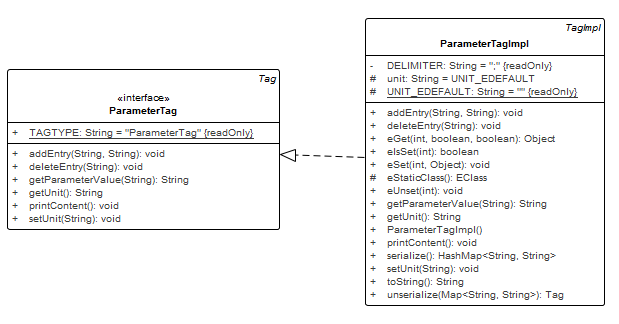
\includegraphics[scale=0.7]{ParameterTag.png}
  		  \caption{Darstellung der Klasse ParameterTagImplung das Interface ParameterTag}
     \label{uml.ParameterTag}
  \end{center}
\end{figure}






\subsubsection{ParameterTag}
Das Interface \textit{ParameterTag} dient als Schnittstelle für den Zugriff auf das Inhalt von ParameterTagImpl. Das Interface erweitert \textit{Tag}. Das \textit{Tag} Interface ist ein in TESTONA allgemein implementiertes Modell, welches auf ein Interface und eine implementierende Klasse basiert (siehe Kapitel \ref{sub.Tags}). In das Interface wird immer das Tagtyp definiert um \textit{Tags} voneinander unterscheiden zu können.

\begin{lstlisting}
public static final String TAGTYPE = "ParameterTag";
\end{lstlisting}

Das \textit{Tag} wurde um die in Abbildung \ref{uml.ParameterTag} zu sehende Methoden erweitert. 

\subsubsection{ParameterTagImpl}
Die Klasse \textit{ParameterTagImpl} erweitert die Klasse \textit{TagImpl} und implementiert \textit{ParameterTag}. In dieser Klasse werden die Vorteile von das Tagmodell deutlicher. Die Klasse \textit{TagImpl} definiert sehr nützliche Methoden und Eigenschaften die in \textit{ParameterTagImpl} weiter angewendet werden.\\

Jedes \textit{Tag} hat als Eigenschaft einen Namen. In diese Klasse entspricht der Name, ein Parametername der aus der Parametertabelle gelesen wurde. Weiterhin ist über \textit{ID} eine eindeutige Identifikationsnummer definiert, um \textit{Tags} des gleichen Typs voneinander zu unterscheiden. Es wurde ein weiteres Attribut implementiert, dass die Einheit (\textit{unit}) des Parameters definiert\\

Der Inhalt von das \textit{Tag} ist durch ein \textit{EcoreEMap<String, String>} definiert. Das erste String ist ein Schlüsselwert und das zweite String der Wert. Im diesem Fall ist der Schlüssel der Name einer Variante, und der Wert ist der Parameterwert des Parameters in dieser Variante. Der Inhalt und Struktur eines \textit{ParameterTags} sieht folgendermaßen aus:\\

\begin{table}[h]
\begin{center}
	\begin{tabular}{|l||ll|}
	 \hline
	 \multicolumn{3}{|c|}{ParameterTag}\\
	 \hline\hline
	 ID			& \multicolumn{2}{|c|}{30}\\
	 \hline
	 Name		& \multicolumn{2}{|c|}{max\_speed}\\
	 \hline
	 Unit		& \multicolumn{2}{|c|}{[km/h]}\\
	 \hline
	 \multirow{5}{*}{Content}	&Key			&Value\\ \cline{2-3}
	 							&Generic		&50\\
	 							&Cabrio		&100\\
	 							&Kombi		&200\\
	 							&Limo		&300\\
	 \hline
	\end{tabular}
	
	\caption{Beispiel eines ParameterTags}
	\label{table:ParameterTagStruktur}
\end{center}
\end{table}


Anhand der Methode \textit{getContent()} kann der Inhalt eines \textit{Tags} aufgerufen werden und mit der Methode \textit{addEntry()} werden Inhalte hinzugefügt. Das Gegenteil kann man mit der Methode \textit{deleteEntry()} erreichen. Wie die Methoden genauer angewendet werden, wird im Listing \ref{lst:CreateParamTag} gezeigt.\\


Sehr relevant sind die Methoden \textit{serialize()} und \textit{unserialize(Map<String, String>)} die für das Schreiben und das Lesen der .testona Datei zuständig sind. Zum Schreiben wird ein \textit{HashMap<String, String>} Objekt zurückgegeben. Das erste \textit{String} beinhaltet der Name des Parameters gefolgt von die Variantennamen. Die Werte sind durch ein Vereinbartes Trennzeichen (;)  getrennt. Das zweite \textit{String} beinhaltet die Einheit des Parameters und die Parameterwerte (in einer geordneten Reihenfolge). Der XML Eintrag für das obige Beispiel (Tabelle \ref{table:ParameterTagStruktur}) wurde wie folgt aussehen:\\

\begin{lstlisting}[caption={XML Darstellung eines ParameterTags}, captionpos=b]
<Tag id="30" type="ParameterTag">
	<Content key="max_speed;Generic;Cabrio;Kombi;Limo" value="km/h;50;100;200;300"/>
<Tag/>
\end{lstlisting}


Beim Laden der .testona Datei erkennt das Programm anhand des Attributs \texttt{type} um welches Typ von \textit{Tag} es sich handelt. Die Methode \textit{unserialize} bekommt als Eingansparameter die in \textit{serialize()} erstellte Zeile als ein \textit{Map<String, String>} Objekt. Durch das Trennzeichen werden die jeweilige Werten voneinander unterschieden und zu den zugehörigen Variablen (name, unit, content) zugeordnet. Beider Vorgänge funktionieren automatisiert dank der Vererbung.

%#######################################################################################
\subsection{ParameterManager}\label{sub:ParameterManager}

\begin{figure}[h!]
  \begin{center}
    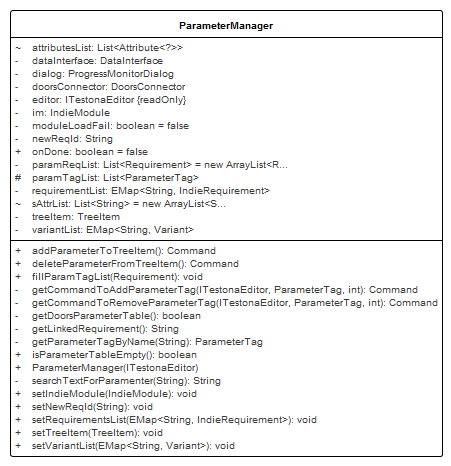
\includegraphics[scale=0.7]{KD_ParameterManager.png}
  		  \caption{Klasse ParameterManager}
     \label{kd.ParameterMananger}
  \end{center}
\end{figure}

Die Klasse \textit{ParameterManager} überprüft und startet die Parameterersetzung. Sie beinhaltet die private innere Klasse \textit{DoorsConnector}, diese kümmert sich um den Verbindungsaufbau mit DOORS und das Laden von den Parameterwerten aus der Parametertabelle. Die Klasse \textit{DoorsConnector} wird genauer in siehe Kapitel \ref{sub.DoorsConn} erklärt.\\


Mit dem Aufruf der Methode \textit{addParameterToTreeItem()} wird die Parameterersetzung gestartet. Die Methode hat als Rückgabewert ein Kommando, indem ein Parameter hinzugefügt oder gelöscht wird (siehe Kapitel \ref{sub.Command}). Als erstes überprüft die Methode ob die an das Baumelement verlinkte Anforderung ein Parameter beinhaltet. Falls kein Parameter in der Anforderung gefunden wurde, gibt die Methode den Wert \textit{null} zurück. Wenn ein Parameter gefunden wurde, wird der Name in einer Variablen gespeichert um es aus DOORS laden zu können. Wenn noch keine Parameter lokal zu Verfügung stehen (in Form von \textit{ParameterTag} innerhalb einer Liste) wird die Verbindung mit DOORS gestartet. Die erforderliche Angaben zum Verbindungsaufbau befinden sich in der Variable \textit{im} vom Typ \textit{IndieModul} (diese wurde von der Klasse \textit{VariantsManager} gesetzt aus das \textit{RequirementsConnectionTag}). Das Objekt der Klasse \textit{DoorsConnetor} hat Zugriff auf \textit{im} und kann die gespeicherte Daten abfragen.\\


Während die Verbindung entsteht und die Parametertabelle geladen wird, wird dem Benutzer ein Dialogfenster angezeigt. Dieser blockiert die Benutzeroberfläche und zeigt ein Fortschrittsbalken. Nach einem erfolgreichen Verbindungsaufbau wird die Parametertabelle geladen. Der Pfad zu der Parametertabelle in DOORS ist als Attribut des Hauptmoduls gespeichert. In das Objekt \textit{im} befindet sich der Pfad zum Hauptmodul. Die aktuell implementierte DOORS API in TESTONA kann nicht diese Attribute abfragen. Eine in Moment in Entwicklungszustand neue API wird in der Lage sein, die Attribute abfragen zu können. An dieser Stelle wurde als Kompromiss eine Konstante angelegt, in der sich der Pfad zur Tabelle befindet.\\

 
Wenn ein Parameter und die zugehörige Werte geladen worden sind, werden sie in \textit{ParameterTag} Objekt gespeichert. Die Methode \texttt{fillParamTagList(Requirement req)} agiert als Parser und wandelt der Übergabeparameter in ein ParameterTag. Zu beachten ist, dass innerhalb DOORS jede Zeile in ein Modul als eine Anforderung betrachtet wird. Danach wurde die Namensgebung vereinbart und der Übergabeparameter ist vom Typ \textit{Requirement}. In das \textit{Requirement} Objekt befinden sich die Variantennamen und die Parameterwerte. Der folgende Quelltextausschnitt kümmert sich im die Speicherung der Parameterwerte in ein \textit{ParameterTag}.\\


\begin{lstlisting}[caption={Auszug von der Erstellung der ParameterTags}, captionpos=b,label={lst:CreateParamTag}]
ParameterTag tempTag = new ParameterTagImpl();
		
for(int i = 0; i < attributesList.size(); i++){
	
	//An der nullte Stelle steht immer der Parametername
	if(i == 0) {
		tempTag.setName(req.getValue(attributesList.get(0)).getValueAsString());
	} else {
		//Füge ein Eintrag hinzu 
		tempTag.addEntry(sAttrList.get(i),
				req.getValue(attributesList.get(i)).getValueAsString());
	}
}
paramTagList.add(tempTag);
\end{lstlisting}


Die Variable \texttt{attributesList} beinhaltet die in DOORS definierten Varianten\footnote{Jede Variante in das DOORS Modul wird als ein Attribut definiert und in einer Spalte angezeigt. Wobei nicht jede Spalte des Moduls ein Attribut ist.}. Die Liste wird iteriert und die Werte werden in das \textit{ParameterTag} gespeichert. Zwei Attribute sind für jedes Parameter in der Liste mindestens definiert. Diese sind der Parametername und ein Standartwert. Möglicherweise ist auch die Einheit des Parameters definiert. Die geladene Werte werden kontrolliert ob sie ungleich ein leerer \textit{String} sind\footnote{Im Ladevorgang einer Anforderung und ihre Attribute in DOORS, wird nicht zwischen leeren und befüllte Zellen unterschieden. Der Rückgabewert ist immer ein \textit{String}. Wenn die Zelle leer ist, wird ein leerer \textit{String} zurückgegeben.}, bevor sie in ein \textit{ParameterTag} gespeichert werden.\\


Wenn alle vorhandenen Varianten für dieses Parameter iteriert worden sind, wird überprüft ob der Inhalt (die Variable \textit{content} des \textit{ParameterTags}) der temporären Variable \texttt{tempTag} nicht leer ist. Es kann vorkommen, dass ein Parameter in das Modul definiert ist, aber keine weitere Informationen wurden ausgefüllt. Wenn Inhalte vorhanden sind, wird das \textit{ParameterTag} zur eine Liste von \textit{ParameterTags} hinzugefügt.\\

Nachdem die Parameter geladen werden konnten und die Liste befühlt ist, wird die Verbindung mit DOORS geschlossen. Das Dialogfenster wird danach geschlossen und die Benutzeroberfläche wird freigegeben. Während dessen wird ein der Liste das richtige \textit{ParameterTag} geladen und die Methode \textit{getCommandToAddParameter()} wird aufgerufen. Diese Methode erzeugt ein Objekt der Klasse \textit{AddParameterTagCommand}. Das zurückgegebene Kommando wird an die Klasse \textit{VariantsManager} weitergeleitet, die wiederum das Kommando an das \textit{ResourSetListener} weitergibt. Dort wird das Kommando verarbeitet.\\


Für den Fall, dass eine Anforderung aus ein Baumelement gelöscht wird, muss zuerst überprüft werden ob die Anforderung ein Parameter beinhaltet. Wenn ein Parameter gefunden worden ist, wird das \textit{ParameterTag} aus dem Baumelement geladen. Mithilfe der Klasse \textit{RemoveParameterTagCommand} wird das \textit{ParameterTag} aus dem Baumelement entfernt.

%#######################################################################################
\subsection{Kommandos}\label{sub.Command}
Für das Hinzufügen bzw. Löschen eines Parameters in einem Baumelement wurden zwei Klassen implementiert, dass aus die Klasse \textit{RecordingCommand} erben. Die Klasse \textit{RecordingCommand} ist eine partielle Implementierung der Klasse \textit{Command}. Diese Klasse nimmt die  Manipulierung der Objekte der Subklasse auf und erzeugt daraus ein Kommando\footnote{14.02.2015; http://download.eclipse.org/modeling/emf/transaction/javadoc/ 1.2.3/org/eclipse/emf/transaction/RecordingCommand.html}. Eine der implementierten Klassen erzeugt ein Kommando für das Hinzufügen eines \textit{ParameterTags} an einem Baumelement\footnote{AddParameterTagCommand}, während der zweiten für das Löschen zuständig ist\footnote{RemoveParameterTagCommand}. Der Konstruktor der beiden Klassen haben die gleichen Parametern. Es werden der aktuelle Editor-Objekt übergeben, sowie das Baumelement ID und das \textit{ParameterTag}.\\


Die Methode \textit{doExecute()} wird überschrieben um die Änderung vorzunehmen. Als erstes werden alle Baumelemente geladen und iteriert bis das Baumelement gefunden wird, dass benötigt wird (anhand er ID). Soll ein \textit{ParameterTag} hinzugefügt werden, dann wird die Methode \textit{addTag(ParameterTag pTag)} aufgerufen.\\


Soll eine \textit{ParameterTag} gelöscht werden, dann wird die Methode \textit{removeTag(ParameterTag pTag)} aufgerufen. Danach muss auch der Name des Baumelementes neu gesetzt werden. Wenn ein Baumelement ein Parameter besitzt, je nach aktive Variante, wird die Darstellung geändert (siehe Kapitel \ref{sec.visialisierung}). Dafür wird der Name des Baumelementes geladen und falls eine Rücksetzung nötig ist, wird diese gemacht. Genaueres dazu wird in Kapitel \ref{sec.LoesungVisualisierung} veranschaulicht.\\

%#######################################################################################
\subsection{Die DOORS Verbindng}\label{sub.DoorsConn}
\subsubsection{DoorsConnector}
%\begin{figure}[h!]
%  \begin{center}
%    \includegraphics[scale=0.7]{.jpg}
%  		  \caption{Darstellung der innere Klasse DoorsConnector in UML}
%     \label{ttn.DoorsConnetor}
%  \end{center}
%\end{figure}

Die private innere Klasse \textit{DoorsConnector} baut die Verbindung zwischen den TESTONA und DOORS auf. Sie implementiert das Interface \textit{IConnectionListener}, dass ein \textit{Listener} für die Verbindung - Events umfasst. Für das Laden von Dateien aus DOORS benötigt die Klasse noch ein \textit{Listener} (IDataListener) und ein \textit{Adapter}(IReqLoadAdapter) \\

Als erstes wird von der Klasse \textit{ParameterManager} die Methode \textit{connectToDoors()} aufgerufen. Diese baut die Verbindung auf, indem gespeicherte Verbindungsdaten aufgerufen werden. Wie bereits in Kapitel \ref{sub:ParameterManager} erwähnt, beinhaltet eine Anforderung die Informationen wo die Anforderung gespeichert ist (welches DOORS Modul und über welches Interface das Modul zu erreichen ist). Für den Verbindungsaufbau werden folgende Objekte benötigt:

\begin{itemize}
\item \textbf{DataInterface: }Über diese Klasse erfolgt die Datenanfrage an DOORS. Die Verbindung wird aufgebaut sowie getrennt. Es werden als erstes die Ordner geladen, danach einzelne Projekte und die nötige Module. Es können verschiedene Darstellungen der Module auch geladen werden (diese müssen in DOORS definiert sein). Hier werden auch direkt einzelne Anforderungen angefragt. Relevant für diese Arbeit ist, dass hiermit das Modul Parametertabelle in DOORS geladen wird.

\item \textbf{PreferenceManagment: } Hier werden die in TESTONA gespeicherte Verbindungsdaten behandelt. Es können Microsoft Access Verbindungensdaten gespeichert werden, aber wir werde nur DOORS betrachten.

\item \textbf{Connector: }beschreibt eine einzelne Verbindung, hat ein \textit{DataIterface}- und \textit{PreferenceManagmentobjekt}

\item \textbf{ConnectionManager: }Singleton. Die Klasse handelt aktive und offene Verbindungen. Hier werden die \textit{ConnectionListeners} und das \textit{DataInterface} für den richtigen \textit{Connector} geregelt.

\end{itemize}


Um die Verbindung mit DOORS aufzubauen muss als erstes die Instanz des \textit{ConnecionManagers} lokal referenziert werden (weil es ein \textit{Singleton} ist, darf kein neues Objekt erzeugt werden). Wenn die Instanz des \textit{ConnectionManagers} geladen ist, kann jetzt der \texttt{connector} aus dem \textit{ConnectionManager} aufgerufen werden.

\begin{lstlisting}[caption={Verbindungsaufbau}, captionpos=b]
try {
	connector = ConnectorManager.getInstance()
				.getConnector(im.getInterId());
	dataInterface = conManager.getNewDataInterface(connector, this);
} catch (ExtensionException e) {
	e.printStackTrace();
}
\end{lstlisting}

 Um dem richtigen \texttt{connector} aufzurufen muss aus das \textit{IndieModul} (\texttt{im.getInterId()}, siehe Kapitel \ref{sub.VariantsManager}) die Interfacekennung als Übergabeparameter angegeben werden. Als nächstes kann über den \textit{ConnectionManager} eines neues \textit{DataInterface} erzeugt werden, wo der \texttt{connector} und das aktuelle Objekt (\textit{DoorsConnector}) übergeben werden.\\
 
Aus den in TESTONA gespeicherte Verbindungspräferenzen werden die Verbindungsparameter für DOORS geladen. An dieser Stelle braucht das \textit{DataInterface} die nötige \textit{Listeners} bevor die Verbindung aufgebaut wird. Durch die Methode \textit{addListener(listener)} wird das \textit{RequirementDataListener} und das \textit{IConnectionListener} (von \textit{DoorsConnetor} implementiert) gesetzt. Mit dem Aufruf der Methode \textit{connecteInterface(Verbindungsparameter)} wird das \textit{DataInterface} an DOORS verbunden.\\

Der Grund warum ein \textit{IConnectionListener} implementiert wird, lautet dass der Verbindungsaufbau in einem neuen Thread stattfindet. Das \textit{DoorsConnetor} Objekt wird über das \textit{IConnectionListener} benachrichtigt ob die Verbindung stattgefunden hat. Die Methode\texttt{interfaceConnected} (aus dem \textit{IConnectionListener}) wird aufgerufen, wenn die Verbindung erfolgreich entstanden ist.

\begin{lstlisting}[caption={Verbindungsaufbau war erfolgreich}, captionpos=b]
@Override
public void interfaceConnected() {
	connected = true;
	reqDataListener.setListener(reqLoadListener);
	dataInterface.loadModule(PARAM_PATH, this, false);
}
\end{lstlisting}

Der gesetzte \textit{RequirementDataListener} benötigt ein \textit{RequirementLoadListener}, dass eine rückmeldung gibt, wenn die Zeilen aus einer Tabelle fertig geladen worden sind. Die Tabelle wird anhand der Methode \texttt{loadModule} wird ein DOORS Modul (Tabelle) geladen. Welches Modul geladen wird, spezifiziert der Parameter \texttt{PARAM\_PATH}. Es gibt an wo sich das Modul in der DOORS Datenbank befindet. Der \textit{RequirementDataListener} erhält die Nachricht, dass ein Modul geladen worden ist. Weiter dazu wird im Kapitel \ref{sub.RequirementDataListener} erläutert.\\


Es wird angenommen, wenn der Benutzer die Parameterersetzung für ein Parameter wahrnimmt, dass er es für weitere Parameter wahrnehmen wird. Da die Datenmenge von einer Parametertabelle relativ gering ist, wurde hier, bezüglich der offene Frage bei dem Lösungsansatz (siehe Kapitel \ref{sec.parameterspeicherung}), die Parametertabelle komplett importiert. 
Ein weiterer Grund lautet, dass nicht für jeder Parameter erneut eine DOORS Verbindgun enstehen muss. So wird die Rechen- und Reaktionszeit von TESTONA so weit es geht gering gehalten. Die Parametertabelle wird erst bei der Verknüpfung von einer Anforderung mit einem Baumelement importiert und nicht beim Import der Anforderungen. 

Wenn die Parametertabelle komplett geladen wurde, ermöglicht die Methode \textit{closeConnection} die Verbindung mit DOORS zu beenden und das \textit{DataInterface} zu schließen.





\subsubsection{RequirementDataListener}\label{sub.RequirementDataListener}

Ist ein Event-Listener, dass auf die Rückmeldung vom Laden eines Moduls wartet. Relevant ist die Methode \texttt{onModuleLoad} die die Zeilen aus der Tabelle liest und speichert.\\

\begin{lstlisting}[caption={Laden der Parametertabelle nach Zeilen}, captionpos=b]
@Override
public void onModuleLoad(Module module, Object family, boolean reload){

	BasicRequirement baseReq;
	saveAttributesNames(module);
				
	for (String reqId : module.getRequirementIds()) {

		baseReq = dataInterface.getRequirement(module, reqId,
				reqLoadListener);

		if (baseReq.checkStatus(BasicRequirement.STATUS_LOADED)){
			paramReqList.add((Requirement) baseReq);
			fillParamTagList((Requirement) baseReq);
		}
	}
	dataInterface.flush(reqLoadListener);
}
\end{lstlisting}

Zu beachten ist, dass in DOORS jede Zeile in einer Tabelle als eine Anforderung (eng. Requirement) gesehen wird. Daher heißen Variablen und Methoden oft \glqq Requirement\grqq~ oder Abkürzung des Wortes (req). Die Methode \texttt{saveAttributesNames} speichert die im geladenes Modul vorhandenen Attribute. Im diesem Fall (treu zum Beispiel mit dem Auto) sind es:

\begin{itemize}\itemsep1pt
\item Paramenter Name
\item Default Value
\item Cabrio Value
\item Kombi Value
\item Limo Value
\end{itemize}

Diese Attribute repräsentieren die Varianten und ein Standardwert, sowie der Name des jeweiligen Parameter. In der Schleife werden alle Zeilen im Modul iteriert und geladen. Wenn die Zeile (\texttt{baseReq}) vollständig geladen wurde, wird diese in der globalen Liste \texttt{paramReqList} als ein \texttt{Requirement} Objekt gespeichert. Die Methode \texttt{fillParamTagList} erzeugt die \textit{ParameterTags} und wurde in Kapitel \ref{sub:ParameterManager} erläutert.\\

Wenn eine Zeile nicht vollständig geladen werden konnte, gibt es das \textit{RequirementLoadListener}, dass sich um das vollständige laden der Zeilen kümmert. Das \textit{RequirementLoadListener} wird in dieser Klasse instantiiert und von der \textit{DoorsConnetor} Klasse gesetzt. Weiter dazu im nächsten Kapitel.


\subsubsection{RequirementLoadListener}\label{sub.RequirementLoadListener}
Der \textit{RequirementLoadListener} reagiert wenn eine Zeile nicht völlstandigt geladen worden ist, und wartet bis diese geladen wird. Die Methode \texttt{onLoad} bekommt als Eingabeparameter eine Liste der nicht geladenen Zeilen.

\begin{lstlisting}[caption={Nachladen der Parametertabelle nach Zeilen}, captionpos=b]
public void onLoad(List<BasicRequirement> requirements) {

	for (BasicRequirement baseReq : requirements) {
		paramReqList.add((Requirement) baseReq);
		fillParamTagList((Requirement) baseReq);
		
	}
}
\end{lstlisting}

Diese Liste wird iteriert und wie in \textit{RequirementDataListener} in der globalen Liste \texttt{paramReqList} als ein \texttt{Requirement} Objekt gespeichert.\\

Weiterhin meldet diese Klasse wenn alle Zeilen aus das DOORS Modul geladen wurden. Das wartenden Dialogfenster aus \ref{sub:ParameterManager} wird benachrichtigt, dass es geschlossen werden kann. Die Benutzeroberfläche von TESTONA ist somit wieder für den Benutzer erreichbar.



%#######################################################################################
%#######################################################################################
\newpage
\section{Darstellung der Parameterwerte}\label{sec.LoesungVisualisierung}
\paragraph{}

Nachdem Parameter in Baumelement vorhanden sind, sollten die Werte angezeigt werden. Wenn ein Pfeil oder die Kombo-Box (siehe Kapitel \ref{sec.visialisierung}) für eine Änderung der Variantenansicht betätigt wird, muss für jedes Baumelement überprüft. Es wird überprüft, ob für die aktive Variante ein Parameterwert definiert worden ist.\\

In \textit{VariantsManager}\\

 \textit{setNamesWithValues} \\
 \textit{executeEMFCommand} \\
 \textit{RenameTreeItemCommand}\\
 \textit{arrangeAll}\\
 
 


%#######################################################################################
%#######################################################################################
\newpage
\section{Testfallgenerierung und Optimierung}
\paragraph{}
Erläuterung der Lösungen zu 4.3